\chapter{Results and Evaluation}
\label{ch:results}

\section{Experimental Setup}

All benchmarks were run on an \textbf{AMD Ryzen 5 7535HS} with 6 physical
cores and 12 logical threads via Simultaneous Multithreading (SMT), clocked
at 2.9\,GHz base with a boost up to 4.6\,GHz, and a 16\,MiB shared L3
cache. The machine had 16\,GiB of DDR5 RAM on a Linux x86\_64 environment.

The runtime was \textbf{OpenJDK 25.0.2} (64-bit Server VM) with
\textbf{Clojure 1.12.4}. Heap size was fixed at 8\,GiB via
\texttt{-Xms8g -Xmx8g} to eliminate dynamic resizing during tests, and
\texttt{-XX:+AlwaysPreTouch} was set to initialize heap pages at JVM startup.
A dedicated \texttt{:bench} profile was used alongside \textbf{Criterium
  0.4.6}, with direct linking enabled and the G1 Garbage Collector active.

Thread counts of 4, 6, and 12 were chosen purposefully: four threads fall
below the physical core count, six match it exactly, and twelve use all
logical threads via SMT.

Two measurement methods were used:

\begin{itemize}
  \item \textbf{Throughput benchmarks} measure committed transactions per
        second (TPS) under concurrent load. All threads are held at a gate
        and released simultaneously to ensure peak contention from the start.
        For scenarios with non-trivial abort rates, aborts per committed
        transaction are also recorded.

  \item \textbf{Latency benchmarks} use Criterium, which runs each scenario
        hundreds of thousands of times on a single thread and reports mean
        execution time with standard deviation. The
        \texttt{transfer-unchecked} variant is used to ensure every iteration
        exercises the full commit path.
\end{itemize}

\section{Throughput and Scalability}

Table~\ref{tab:throughput-summary} summarizes throughput across all scenarios
and thread counts.

\begin{table}[H]
  \centering
  \caption{Throughput summary across all scenarios and thread counts.
    Aborts/commit is reported only for scenarios where conflicts were
    observed.}
  \label{tab:throughput-summary}
  \begin{tabular}{@{}l r r r r r@{}}
    \toprule
    \textbf{Scenario}     &
    \textbf{4T (TPS)}     &
    \textbf{6T (TPS)}     &
    \textbf{12T (TPS)}    &
    \textbf{Scaling}      &
    \textbf{Aborts/commit}                                                                                 \\
                          &           &           &           & $\mathbf{4T{\to}12T}$ & \textbf{(4/6/12)}  \\
    \midrule
    High Contention       & 138,633   & 253,421   & 425,973   & $3.07\times$          & 0.00 / 0.00 / 0.00 \\
    Low Contention        & 1,322,570 & 1,092,815 & 1,033,984 & $0.78\times$          & ---                \\
    Bank Transfer         & 213,631   & 163,402   & 173,725   & $0.81\times$          & ---                \\
    Read-Heavy (10\% w.)  & 533,885   & 1,082,057 & 1,969,463 & $3.69\times$          & ---                \\
    Write-Heavy (90\% w.) & 637,709   & 418,108   & 257,574   & $0.40\times$          & 0.00 / 0.00 / 0.00 \\
    \bottomrule
  \end{tabular}
\end{table}

\subsection{High Contention}

All threads compete for a single shared reference, each incrementing a global
counter inside a transaction. Every pair of concurrent transactions conflicts,
and at most one can commit at a time: the worst case for any optimistic
concurrency system.

Despite this, throughput scales from 138,633\,TPS at 4 threads to
253,421\,TPS at 6 threads ($1.83\times$) and 425,973\,TPS at 12 threads
($3.07\times$). Abort rates at the commit phase are zero at every thread
count: conflicts are caught at write time by the ownership protocol, so no
transaction ever reaches commit and fails there.

\begin{figure}[H]
  \centering
  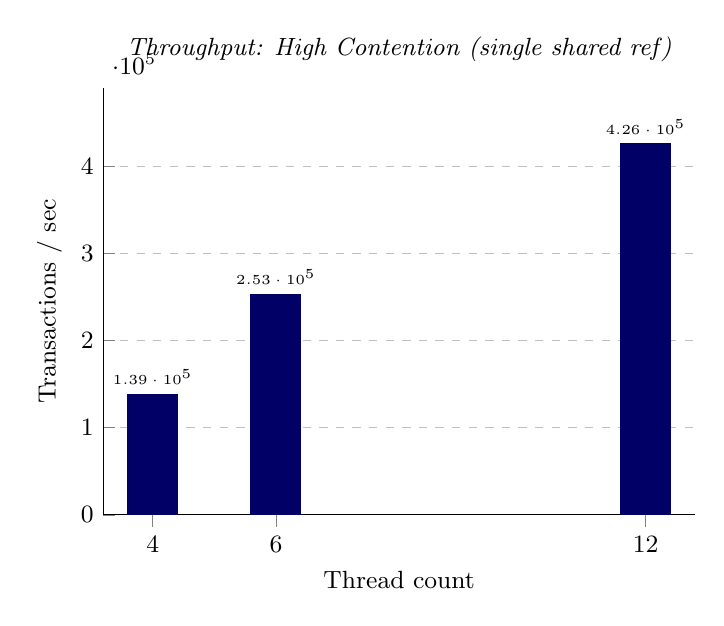
\begin{tikzpicture}
    \begin{axis}[
        title={Throughput: High Contention (single shared ref)},
        xlabel={Thread count}, ylabel={Transactions / sec},
        ybar, bar width=18pt, width=0.75\textwidth, height=7cm,
        xtick=data, ymin=0, enlarge y limits={upper, value=0.15},
        ymajorgrids=true, grid style=dashed,
        nodes near coords, nodes near coords align={vertical},
        every node near coord/.append style={font=\tiny, anchor=south},
        tick label style={font=\small}, label style={font=\small},
        title style={font=\small\itshape}, clip=false,
        axis y line*=left, axis x line*=bottom,
      ]
      \addplot[fill=blue!40!black, draw=blue!40!black] coordinates {
          (4,138633) (6,253421) (12,425973)
        };
    \end{axis}
  \end{tikzpicture}
  \caption{Throughput under maximal conflict. All threads write the same
    reference. Throughput scales from 139K to 426K\,TPS with zero commit-phase
    aborts at every thread count.}
  \label{fig:throughput-high-contention}
\end{figure}

\subsection{Low Contention}

Each thread works on its own private reference and never touches another
thread's data. There are no conflicts by construction, so every transaction
commits on its first attempt. This measures the baseline cost of the commit
path itself.

Throughput is 1,322,570\,TPS at 4 threads and falls to 1,092,815\,TPS at 6
threads and 1,033,984\,TPS at 12 threads. Even with no data conflicts, every
write transaction must acquire the global commit lock, so adding threads
creates a queue at that lock rather than useful parallelism. The JFR profiling
data in Section~\ref{sec:bottlenecks} confirms that all blocking in this
scenario is on that one lock.

\begin{figure}[H]
  \centering
  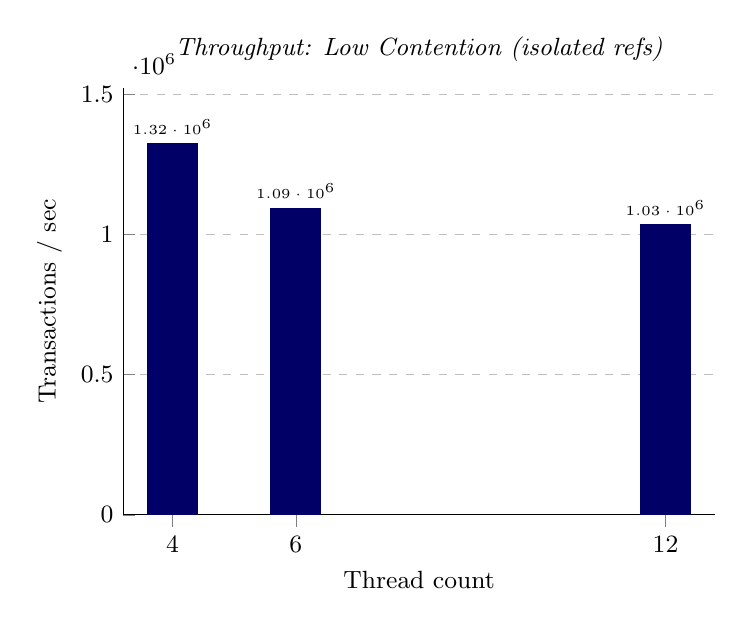
\begin{tikzpicture}
    \begin{axis}[
        title={Throughput: Low Contention (isolated refs)},
        xlabel={Thread count}, ylabel={Transactions / sec},
        ybar, bar width=18pt, width=0.75\textwidth, height=7cm,
        xtick=data, ymin=0, enlarge y limits={upper, value=0.15},
        ymajorgrids=true, grid style=dashed,
        nodes near coords, nodes near coords align={vertical},
        every node near coord/.append style={font=\tiny, anchor=south},
        tick label style={font=\small}, label style={font=\small},
        title style={font=\small\itshape}, clip=false,
        axis y line*=left, axis x line*=bottom,
      ]
      \addplot[fill=blue!40!black, draw=blue!40!black] coordinates {
          (4,1322570) (6,1092815) (12,1033984)
        };
    \end{axis}
  \end{tikzpicture}
  \caption{Throughput when each thread works on its own isolated reference.
    The declining profile reflects commit-lock queuing even under zero data
    contention.}
  \label{fig:throughput-low-contention}
\end{figure}

\subsection{Bank Transfer}

Threads randomly pick pairs of accounts from a shared pool of 20 and transfer
a random amount, committing only when the source account has sufficient funds.
Contention arises naturally since accounts are shared across all threads.

Throughput peaks at 213,631\,TPS at 4 threads and drops to 163,402\,TPS at
6 threads, recovering slightly to 173,725\,TPS at 12 threads. The decline
follows the same pattern as the low-contention scenario: nearly every
transaction writes to two accounts and must acquire the global commit lock,
which becomes the bottleneck as thread count grows.

Correctness is verified after each run by checking that the total balance
across all accounts equals the starting sum, which holds in every measurement.

\begin{figure}[H]
  \centering
  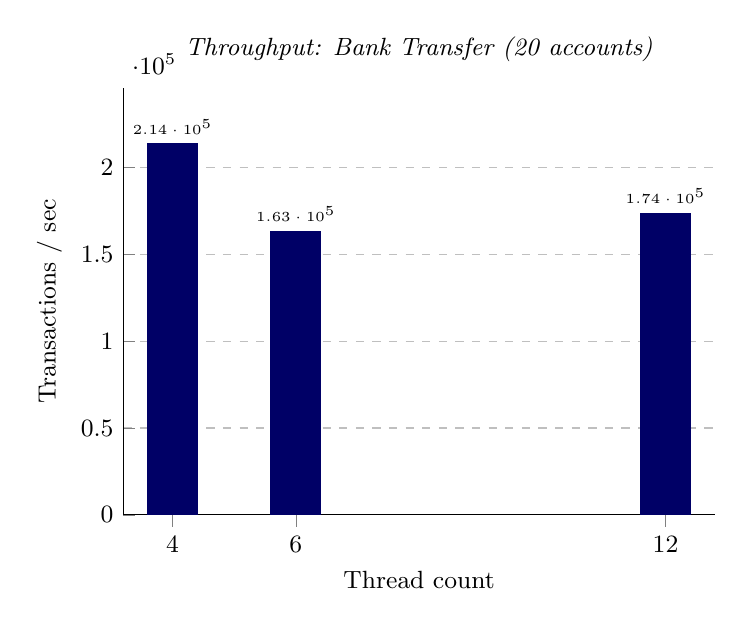
\begin{tikzpicture}
    \begin{axis}[
        title={Throughput: Bank Transfer (20 accounts)},
        xlabel={Thread count}, ylabel={Transactions / sec},
        ybar, bar width=18pt, width=0.75\textwidth, height=7cm,
        xtick=data, ymin=0, enlarge y limits={upper, value=0.15},
        ymajorgrids=true, grid style=dashed,
        nodes near coords, nodes near coords align={vertical},
        every node near coord/.append style={font=\tiny, anchor=south},
        tick label style={font=\small}, label style={font=\small},
        title style={font=\small\itshape}, clip=false,
        axis y line*=left, axis x line*=bottom,
      ]
      \addplot[fill=blue!40!black, draw=blue!40!black] coordinates {
          (4,213631) (6,163402) (12,173725)
        };
    \end{axis}
  \end{tikzpicture}
  \caption{Throughput under a realistic mixed workload with 20 shared
    accounts. Throughput peaks at 4 threads and declines at higher counts,
    consistent with the global commit lock being the bottleneck.}
  \label{fig:throughput-bank-transfer}
\end{figure}

\subsection{Read-Heavy and Write-Heavy Workloads}
\label{sec:read-write-heavy}

Both scenarios use a mixed workload over 10 shared references.

\paragraph{Read-Heavy (10\% writes).}
Each transaction either writes a randomly chosen reference (10\% probability)
or reads and sums all 10 references (90\% probability). Read-only transactions
skip the commit lock entirely, reading a consistent snapshot directly from the
version history.

This is the key advantage of the MVCC design. Throughput scales from
533,885\,TPS at 4 threads to 1,082,057\,TPS at 6 threads ($2.03\times$) and
1,969,463\,TPS at 12 threads ($3.69\times$): the strongest scaling result
in the suite and the clearest demonstration of the MVCC benefit.

\paragraph{Write-Heavy (90\% writes).}
With 90\% of transactions writing, nearly every transaction must acquire the
commit lock. Throughput falls monotonically: 637,709\,TPS at 4 threads,
418,108\,TPS at 6 threads ($0.66\times$), and 257,574\,TPS at 12 threads
($0.40\times$). Abort rates are zero throughout, ruling out retries as a
factor. The bottleneck is entirely the commit lock, confirmed by the JFR data
in Section~\ref{sec:bottlenecks}.

\begin{figure}[H]
  \centering
  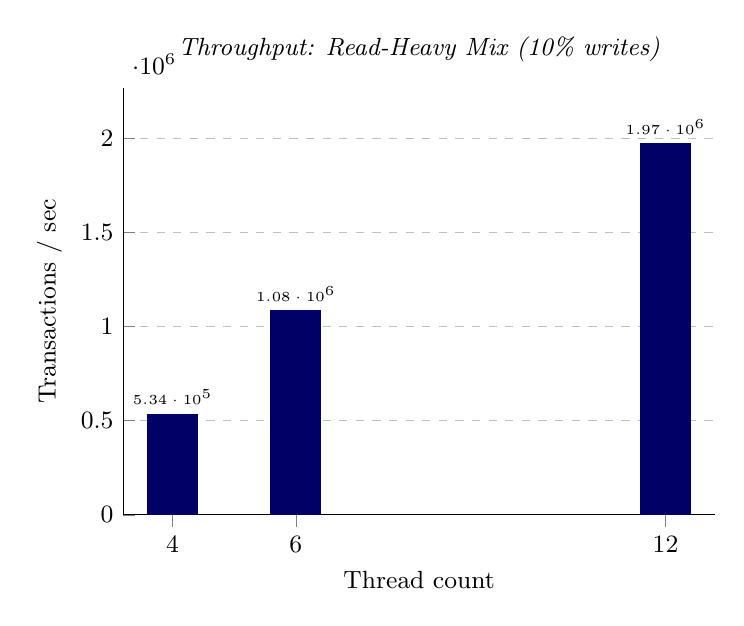
\begin{tikzpicture}
    \begin{axis}[
        title={Throughput: Read-Heavy Mix (10\% writes)},
        xlabel={Thread count}, ylabel={Transactions / sec},
        ybar, bar width=18pt, width=0.75\textwidth, height=7cm,
        xtick=data, ymin=0, enlarge y limits={upper, value=0.15},
        ymajorgrids=true, grid style=dashed,
        nodes near coords, nodes near coords align={vertical},
        every node near coord/.append style={font=\tiny, anchor=south},
        tick label style={font=\small}, label style={font=\small},
        title style={font=\small\itshape}, clip=false,
        axis y line*=left, axis x line*=bottom,
      ]
      \addplot[fill=blue!40!black, draw=blue!40!black] coordinates {
          (4,533885) (6,1082057) (12,1969463)
        };
    \end{axis}
  \end{tikzpicture}
  \caption{Throughput with 90\% read-only transactions. Readers access
    consistent snapshots without the commit lock, so additional threads
    contribute genuine parallelism. Throughput scales to 1.97M\,TPS at
    12 threads.}
  \label{fig:throughput-read-heavy}
\end{figure}

\begin{figure}[H]
  \centering
  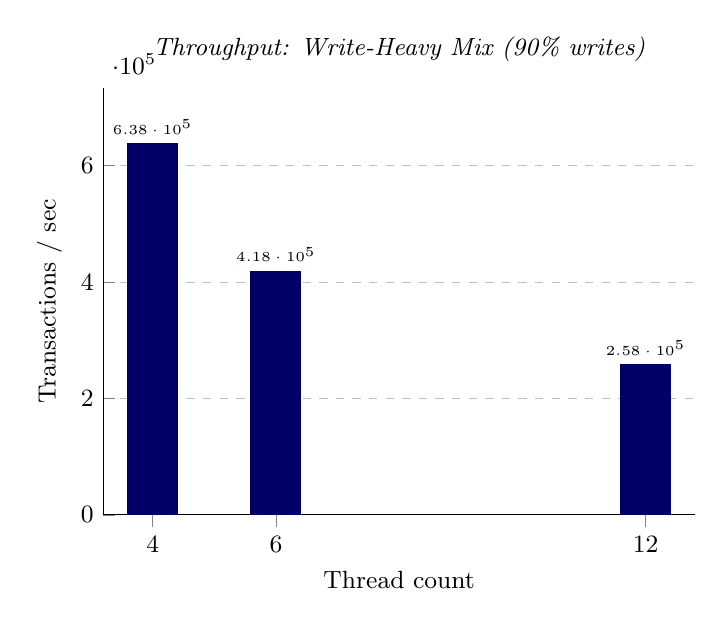
\begin{tikzpicture}
    \begin{axis}[
        title={Throughput: Write-Heavy Mix (90\% writes)},
        xlabel={Thread count}, ylabel={Transactions / sec},
        ybar, bar width=18pt, width=0.75\textwidth, height=7cm,
        xtick=data, ymin=0, enlarge y limits={upper, value=0.15},
        ymajorgrids=true, grid style=dashed,
        nodes near coords, nodes near coords align={vertical},
        every node near coord/.append style={font=\tiny, anchor=south},
        tick label style={font=\small}, label style={font=\small},
        title style={font=\small\itshape}, clip=false,
        axis y line*=left, axis x line*=bottom,
      ]
      \addplot[fill=blue!40!black, draw=blue!40!black] coordinates {
          (4,637709) (6,418108) (12,257574)
        };
    \end{axis}
  \end{tikzpicture}
  \caption{Throughput when 90\% of transactions write. The monotonically
    declining profile, combined with zero abort rates, confirms the commit
    lock as the sole bottleneck.}
  \label{fig:throughput-write-heavy}
\end{figure}

\section{Version History Size}
\label{sec:history-sweep}

Each reference keeps a short history of past values so that concurrent readers
can always find a consistent snapshot. A history that is too short causes reads
to fail when no valid snapshot exists (a \emph{trim abort}); one that is too
long increases read latency and generates more short-lived allocations per
commit, increasing garbage collection overhead. To characterize this
trade-off, the bank transfer scenario was repeated across history sizes of 8,
16, 32, 64, 128, and 256 at thread counts of 4, 6, and 12, with 50,000
transactions per thread.

\begin{table}[H]
  \centering
  \caption{Version history size sweep: bank transfer throughput and abort
    rates (20 accounts, 50{,}000 transactions per thread).}
  \label{tab:history-sweep}
  \begin{tabular}{@{}r r r r r@{}}
    \toprule
    \textbf{\texttt{max-history}}   & \textbf{Threads}            & \textbf{TPS} &
    \textbf{Conflict aborts/commit} & \textbf{Trim aborts/commit}                              \\
    \midrule
    8                               & 4                           & 405,530      & 0.17 & 0.00 \\
    8                               & 6                           & 518,980      & 0.15 & 0.00 \\
    8                               & 12                          & 328,653      & 0.33 & 0.00 \\
    \midrule
    16                              & 4                           & 532,988      & 0.15 & 0.00 \\
    16                              & 6                           & 475,417      & 0.15 & 0.00 \\
    16                              & 12                          & 276,301      & 0.41 & 0.00 \\
    \midrule
    32                              & 4                           & 505,626      & 0.10 & 0.00 \\
    32                              & 6                           & 526,794      & 0.14 & 0.00 \\
    32                              & 12                          & 318,387      & 0.34 & 0.00 \\
    \midrule
    64                              & 4                           & 518,794      & 0.13 & 0.00 \\
    64                              & 6                           & 454,909      & 0.18 & 0.00 \\
    64                              & 12                          & 322,807      & 0.33 & 0.00 \\
    \midrule
    128                             & 4                           & 515,565      & 0.13 & 0.00 \\
    128                             & 6                           & 520,253      & 0.15 & 0.00 \\
    128                             & 12                          & 250,567      & 0.48 & 0.00 \\
    \midrule
    256                             & 4                           & 494,023      & 0.13 & 0.00 \\
    256                             & 6                           & 502,525      & 0.12 & 0.00 \\
    256                             & 12                          & 226,295      & 0.49 & 0.00 \\
    \bottomrule
  \end{tabular}
\end{table}

Three results stand out.

First, trim aborts are zero across all history sizes and thread counts. The
bank transfer workload distributes writes across 20 accounts, so any single
reference is written infrequently relative to how fast history slots cycle. A
transaction's read point is always recent enough that \texttt{find-entry}
locates a valid snapshot. Trim aborts would appear in workloads that
concentrate writes on very few references, where a single ref could accumulate
enough commits to exhaust the history window before a concurrent reader
accesses it.

Second, history size has no consistent effect on throughput at 4 and 6 threads
across the range 8-256.

Third, at 12 threads throughput drops at sizes 128 and 256, falling from the
318,000-328,000\,TPS range seen at sizes 8-64 to 250,567 and 226,295\,TPS.
This is the only consistent directional effect in the table. The cause is
that \texttt{apply-writes!} appends a new entry to the history vector on every
commit via \texttt{conj}, and at sizes 128 and 256 these vectors are large
enough that the resulting allocation and GC cost becomes visible at 12 threads. 
At 4 and 6 threads the commit rate is lower and the overhead is not significant.

Conflict abort rates at 12 threads are elevated throughout (0.33-0.49),
consistent with the commit-lock pressure described in
Section~\ref{sec:bottlenecks}, but show no reliable correlation with history
size.

\begin{figure}[H]
  \centering
  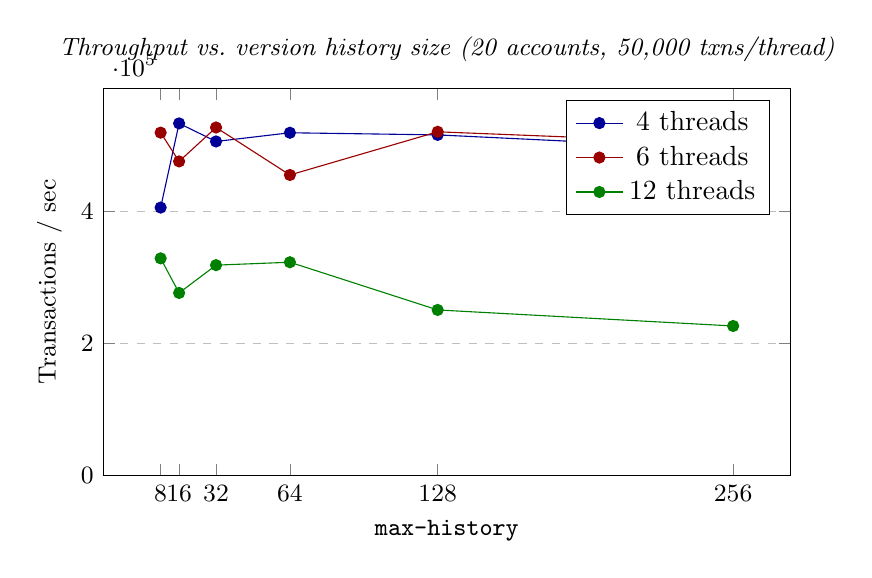
\begin{tikzpicture}
    \begin{axis}[
        title={Throughput vs.\ version history size (20 accounts,
            50{,}000 txns/thread)},
        xlabel={\texttt{max-history}},
        ylabel={Transactions / sec},
        width=0.85\textwidth, height=6.5cm,
        xtick={8,16,32,64,128,256},
        ymin=0,
        ymajorgrids=true, grid style=dashed,
        mark=*, tick label style={font=\small},
        label style={font=\small}, title style={font=\small\itshape},
        legend pos=north east,
      ]
      \addplot[color=blue!60!black, mark=*] coordinates {
          (8,405530) (16,532988) (32,505626) (64,518794) (128,515565) (256,494023)
        };
      \addlegendentry{4 threads}
      \addplot[color=red!60!black, mark=*] coordinates {
          (8,518980) (16,475417) (32,526794) (64,454909) (128,520253) (256,502525)
        };
      \addlegendentry{6 threads}
      \addplot[color=green!50!black, mark=*] coordinates {
          (8,328653) (16,276301) (32,318387) (64,322807) (128,250567) (256,226295)
        };
      \addlegendentry{12 threads}
    \end{axis}
  \end{tikzpicture}
  \caption{Throughput across version history sizes at 50,000 transactions per
    thread. At 4 and 6 threads throughput is flat across all sizes. At 12
    threads it declines at sizes 128 and 256 due to GC overhead from large
    history vectors. Trim aborts are zero throughout.}
  \label{fig:history-sweep}
\end{figure}

\section{Latency Analysis}

Figure~\ref{fig:bank-contention-latency} shows mean transaction latency across
four scenarios on a logarithmic scale. The logarithmic axis is necessary
because the extreme-contention case is roughly two orders of magnitude slower
than the no-contention baseline.

\paragraph{Scenario (i): single uncontended transfer.}
A single transfer between two fixed accounts with no concurrent threads. This
is the baseline cost of a complete commit: reading the current value, preparing
the write, acquiring the lock, validating reads, applying the write, and
dispatching any registered callbacks. Baseline latency is
\textbf{1.76\,$\mu$s} ($\pm$\,0.03).

\paragraph{Scenario (ii): extreme contention.}
Multiple concurrent threads all target the same two accounts simultaneously.
Latency rises to \textbf{401.56\,$\mu$s} ($\pm$\,35.25), a $228\times$
increase. The large standard deviation (about 9\% of the mean) reflects how
long a thread has to wait before retrying after a conflict.

\paragraph{Scenarios (iii) and (iv): callback overhead.}
These scenarios measure the cost of \texttt{on-commit} callbacks,
single-threaded with no concurrency. Scenario~(iii) is the no-callback
baseline at \textbf{1.59\,$\mu$s} ($\pm$\,0.03); scenario~(iv) adds a
callback at \textbf{1.81\,$\mu$s} ($\pm$\,0.08). The difference,
\textbf{0.22\,$\mu$s}, is the cost of dispatching the callback, roughly
14\% of the baseline commit cost. The small difference between scenarios~(i)
and~(iii) (1.76 vs.\ 1.59\,$\mu$s) is within normal measurement variation
between separate Criterium runs.

\begin{figure}[htbp]
  \centering
  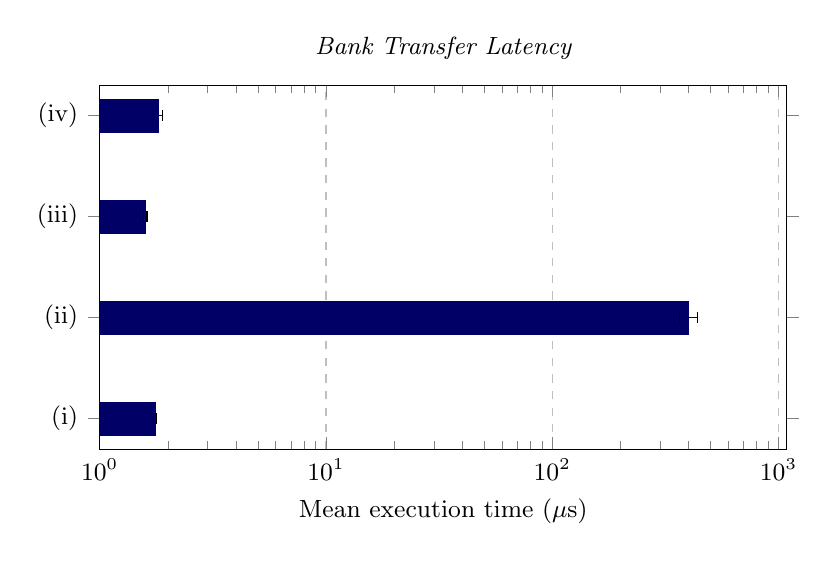
\begin{tikzpicture}
    \begin{axis}[
        title={Bank Transfer Latency},
        xlabel={Mean execution time ($\mu$s)},
        width=0.85\textwidth, height=6.2cm,
        xbar, bar width=12pt, xmode=log, xmin=1,
        enlarge x limits={upper, value=0.15},
        ytick={0,1,2,3},
        yticklabels={(\romannumeral 1),(\romannumeral 2),(\romannumeral 3),(\romannumeral 4)},
        xmajorgrids=true, grid style=dashed,
        tick label style={font=\small}, label style={font=\small},
        title style={font=\small\itshape},
      ]
      \addplot[fill=blue!40!black, draw=blue!40!black,
        error bars/.cd, x dir=both, x explicit
      ] coordinates {
          (1.758,0) +- (0.030,0)
          (401.556,1) +- (35.249,0)
          (1.587,2) +- (0.032,0)
          (1.810,3) +- (0.077,0)
        };
    \end{axis}
  \end{tikzpicture}
  \vspace{0.5em}
  \begin{minipage}{0.85\textwidth}
    \centering \small
    \begin{tabular}{@{}r l@{}}
      (\romannumeral 1) & single transfer, no concurrency                   \\
      (\romannumeral 2) & same transfer under extreme concurrent load       \\
      (\romannumeral 3) & single transfer, no callback registered           \\
      (\romannumeral 4) & single transfer, with \texttt{on-commit} callback \\
    \end{tabular}
  \end{minipage}
  \caption{Bank transfer latency on a logarithmic axis. Scenarios~(i) and
    (iii)--(iv) are single-threaded; scenario~(ii) uses concurrent threads
    all targeting the same two accounts.}
  \label{fig:bank-contention-latency}
\end{figure}

\section{Discussion}

\subsection{Architectural Strengths}

The results confirm two clear strengths of the design.

The first is the MVCC read path. Read-only transactions never acquire any
lock, they read a consistent snapshot directly from the version history.
This is why the read-heavy scenario scales to 1,969,463\,TPS at 12 threads
($3.69\times$ from 4 threads), outperforming every other scenario at high
thread counts and being the only scenario in the suite to scale beyond the
physical core count.

The second is the low overhead of \texttt{on-commit} callbacks: 0.22\,$\mu$s,
or roughly 14\% of the single-threaded baseline. Side-effect coordination can
be added to the transactional model without meaningful overhead.

Abort rates are zero across all throughput scenarios. Even under maximum
contention, conflicts are caught at write time by the ownership protocol, so
no transaction ever reaches commit and fails there.

\subsection{Identified Bottleneck: the Commit Lock}
\label{sec:bottlenecks}

The dominant bottleneck across all write-heavy scenarios is the \textbf{global
  commit lock}. Every write transaction must acquire it to record its result.
When multiple threads compete for it, they queue and wait, directly reducing
throughput.

The JFR profiling data makes this concrete. In the write-heavy scenario, a
single lock accounts for all thread blocking in the process.
Table~\ref{tab:jfr-summary} shows total time threads spent waiting for that
lock at each thread count.

\begin{table}[H]
  \centering
  \caption{JFR commit-lock profiling: write-heavy scenario. All blocking is
    concentrated on a single lock. The 12-thread run shows a second lock with
    one brief event, accounting for 3\% of total blocked time.}
  \label{tab:jfr-summary}
  \begin{tabular}{@{}r r r r r@{}}
    \toprule
    \textbf{Threads}              &
    \textbf{Total wait (B ticks)} &
    \textbf{Avg wait (M ticks)}   &
    \textbf{Max wait (M ticks)}   &
    \textbf{Lock events}                                  \\
    \midrule
    4                             & 1.54 & 110 & 163 & 14 \\
    6                             & 2.81 & 134 & 183 & 21 \\
    12                            & 5.55 & 121 & 186 & 46 \\
    \bottomrule
  \end{tabular}
\end{table}

Two observations follow.

First, total wait time grows faster than thread count. Going from 4 to 12
threads ($3\times$ more workers) causes total wait time to grow $3.6\times$,
from 1.54\,B to 5.55\,B ticks. This is the signature of a saturated lock:
each new thread makes every other thread wait longer.

Second, the maximum wait per event is stable across thread counts
(163-186\,M ticks). Individual commits are not slower at higher concurrency;
threads simply queue for longer. This means replacing the single global lock
with per-reference or per-stripe locks would recover the lost throughput
without changing how commits work internally.

This directly motivates the per-stripe commit lock discussed in
Section~\ref{sec:future}.